\documentclass[10pt]{article}

\usepackage[margin=0.78in]{geometry}
\usepackage{amsmath,amssymb,mathtools}
\usepackage{booktabs,longtable,tabularx,array,multirow}
\usepackage{graphicx}
\usepackage{xcolor}
\usepackage{microtype}
\usepackage{enumitem}
\usepackage{caption}
\usepackage{fancyhdr}
\usepackage[hidelinks]{hyperref}
\usepackage{xurl}
\usepackage{xspace}

\definecolor{sidblue}{HTML}{174A7E}
\definecolor{sidlight}{HTML}{EAF1F8}
\definecolor{sidred}{HTML}{8E2C2C}
\definecolor{sidgreen}{HTML}{2C6E49}
\definecolor{sidgray}{HTML}{5D6570}

\hypersetup{
  colorlinks=true,
  linkcolor=sidblue,
  citecolor=sidblue,
  urlcolor=sidblue,
  pdftitle={A Unified SID Program: Theory, Synthetic Evidence, and the Next Decisive Experiments},
  pdfauthor={diffusionCircuit project synthesis}
}

\setlist[itemize]{leftmargin=1.35em,itemsep=2pt,topsep=4pt}
\setlist[enumerate]{leftmargin=1.55em,itemsep=3pt,topsep=4pt}
\setlength{\parindent}{0pt}
\setlength{\parskip}{5pt}
\renewcommand{\arraystretch}{1.16}

\pagestyle{fancy}
\fancyhf{}
\lhead{Unified SID synthesis}
\rhead{12 July 2026}
\cfoot{\thepage}
\setlength{\headheight}{13pt}

\newcommand{\Ph}{P_h}
\newcommand{\E}{\mathbb{E}}
\newcommand{\R}{\mathbb{R}}
\newcommand{\given}{\,\middle|\,}
\newcommand{\nise}{\operatorname{nISE}}
\newcommand{\nrmse}{\operatorname{NRMSE}}
\newcommand{\SIDQ}{\textnormal{\textsc{SID-Q}}\xspace}
\newcommand{\FiniteSID}{\textnormal{\textsc{Finite-SID}}\xspace}
\newcommand{\DiffSID}{\textnormal{\textsc{Diffusion-SID}}\xspace}
\newcommand{\SBTGK}{\textnormal{\textsc{SBTG-K}}\xspace}
\newcommand{\CPSID}{\textnormal{\textsc{CP-SID}}\xspace}
\newcommand{\yes}{\textcolor{sidgreen}{yes}}
\newcommand{\no}{\textcolor{sidred}{no}}

\newenvironment{takeaway}
  {\begin{quote}\color{sidblue}\textbf{Bottom line.}\ }
  {\end{quote}}

\title{\vspace{-1.2cm}\textbf{A Unified SID Program}\\[3pt]
\large Theory, synthetic evidence, failure modes, and the next decisive experiments}
\author{Internal methods synthesis for the diffusionCircuit project}
\date{12 July 2026}

\begin{document}

\maketitle

\begin{abstract}
The project has accumulated several methods that initially look separate: quadratic score-based interaction discovery, the original score-based temporal graph operator, point-history tangents, finite history contrasts, conditional diffusion, and channel-specific changepoint scans. They are better understood as components of one program. The population object is the observed conditional predictive law \(h\mapsto P(Y\mid H=h)\). A predictive backend represents that law by a normalized density, an outcome score, a joint-state score, or samples. An adapter converts the representation into a supported history contrast or derivative. A typed readout declares whether the target is mean, dispersion, covariance, interaction, skewness, or tail behavior. A calibrated inference layer can then detect static structure or temporal changes.

This synthesis audits the recent synthetic experiments under that decomposition. The empirical conclusion is candid. Normalized likelihood and classical sparse dynamics remain the leaders when their models are tractable and approximately correct. Current score objectives have not produced a general performance advantage. Finite contrasts are nevertheless genuinely promising for location changes and low-rank mixture interactions, and they provide the cleanest generalization of the SID idea beyond a quadratic law. Covariance-only and skew-only contrasts, synaptic-gating readouts, and mechanism-specific SBTG localization currently fail their relevant zero or classical baselines. Conditional diffusion is therefore best treated as a flexible backend for sample-only or intractably normalized laws, not as the scientific claim itself. Changepoint detection is a downstream wrapper and should only be used for channels that pass static oracle and learned-model gates.

The recommended research direction is \emph{finite, typed, support-aware SID}: learn the best available predictive generator; form an exact finite signed contrast at a scientifically declared perturbation scale; estimate bounded or projected witnesses through multiple routes; and report channel-specific functionals with route-agreement and mechanism-confusion controls. The report ends with a staged, preregistered experiment program designed to determine whether this framework has an impactful regime rather than merely a coherent notation.
\end{abstract}

\tableofcontents
\newpage

\section{Executive verdict}

\begin{takeaway}
There is no evidence that a score or diffusion objective is currently the best general estimator of conditional dynamics. The best-developed original idea is the finite-contrast SID architecture, because it preserves the score-based sensitivity interpretation while allowing normalized densities, classifiers, scores, or samples as interchangeable backends. It already works for location and low-rank mixture changes. Its next scientific test is whether redesigned adapters can recover covariance and skew at the oracle level and whether a flexible score/sample backend wins in a regime where likelihood is unavailable or misspecified.
\end{takeaway}

The main conclusions are:

\begin{enumerate}
  \item \textbf{The methods are not six independent theories.} They share one population object, \(P_h=P(Y\mid H=h)\), and differ mainly in representation, adapter, readout, and inference layer.
  \item \textbf{SID should be the umbrella, not the quadratic implementation.} The current closed-form quadratic model is denoted \SIDQ. It is one convenient score-matching backend with Gaussian reconstruction, not the definition of SID.
  \item \textbf{Finite contrasts are the most promising core.} They define an exact, supported comparison of predictive laws and can be estimated from densities, density ratios, classification, scores, or samples. This is the natural generalization of infinitesimal SID.
  \item \textbf{SBTG is a derivative/localization route, not a separate mechanism estimator.} Its ideal mixed operator is \(K_v=D_v\nabla_y\log p_h=\nabla_y D_v\log p_h\). Recovering the history witness from this gradient requires integration, centering, support, and boundary conditions. Current empirical SBTG statistics are reduced-form screens and are not mechanism-specific.
  \item \textbf{Diffusion is a backend.} It is useful if the law is complex, the normalizer is unavailable, or sampling is required. Denoising score matching targets a corrupted outcome score; it does not by itself identify the clean history derivative or a physical mechanism.
  \item \textbf{Changepoints are an inference wrapper.} A changepoint scan can be applied to a validated mean, variance, tail, or general-law statistic. It does not rescue an invalid static channel.
  \item \textbf{Current wins are narrow but real.} Finite signed classifiers/ratios recover location changes, and ratio critics recover low-rank mixture interactions. Mean and matched-tail changepoint probes work strongly in matched settings.
  \item \textbf{Current failures are structural, not just optimization failures.} Covariance and skew adapters fail even with oracle samples; score risk does not control history-derivative error; gating readouts lose to the zero field; and SBTG dispersion statistics barely exceed chance.
\end{enumerate}

\subsection{What should carry the project forward}

The project should be organized around the following stack:
\[
\begin{aligned}
\text{predictive law/generator}
&\longrightarrow \text{finite supported contrast}
\longrightarrow \text{bounded or projected witness}\\
&\longrightarrow \text{typed channel readout}
\longrightarrow \text{calibrated inference}.
\end{aligned}
\]

The specific working hypothesis is not ``diffusion beats likelihood.'' It is:

\begin{quote}
When the conditional law is sufficiently non-Gaussian or only available through a sampler/score, finite supported contrast adapters can expose scientifically useful history sensitivities that simple mean models and generic two-sample tests cannot localize, while retaining controlled claims and calibration.
\end{quote}

That hypothesis remains plausible, but it has not yet been demonstrated in the hard channels or in a regime where the flexible backend is necessary.

\section{One mathematical object, four layers}

\subsection{The population object}

Let \(H\in\mathcal H\) denote an observed history or conditioning state and \(Y\in\mathcal Y\subseteq\R^d\) the future response. The basic object is the conditional predictive law
\[
  \Ph(A)=\Pr(Y\in A\mid H=h), \qquad A\subseteq\mathcal Y.
\]
When a density exists, write \(p_h(y)\). This object is observed-law and predictive. Without further intervention, invariance, sufficiency, or structural assumptions, it is not automatically a causal mechanism.

Every current non-latent method can be placed in four layers.

\begin{center}
\begin{tabularx}{\linewidth}{@{}p{0.14\linewidth}X X@{}}
\toprule
Layer & Question & Examples in the project \\
\midrule
Representation & How is \(P_h\) learned or accessed? & Gaussian/Student-\(t\)/MDN density; conditional outcome score; joint-state score; diffusion sampler; oracle simulator \\
Adapter & How are two nearby histories compared? & Autodifferentiation; finite density ratio; signed classifier; Riesz projection; score difference; mixed SBTG operator \\
Readout & Which aspect of the response law is the target? & Mean, variance, covariance, low-rank interaction, skewness, tail probability, local occupancy \\
Inference & How is uncertainty or temporal change declared? & Bootstrap, held-out route agreement, CUSUM/GLR, calibrated windows, changepoint localization \\
\bottomrule
\end{tabularx}
\end{center}

This separation prevents three recurrent category errors: comparing a graph score with a conditional density by one scalar; treating a native training loss as proof of downstream derivative accuracy; and interpreting a detected distributional change as a specific mechanism.

\subsection{Infinitesimal history sensitivity}

Let \(T_{\epsilon,v}h\) perturb history \(h\) in a declared direction \(v\). If differentiability and common-support conditions hold, define the history score or infinitesimal SID witness
\[
  \ell_v(y;h)
  =D_v\log p_h(y)
  =\left.\frac{\partial}{\partial\epsilon}
  \log p_{T_{\epsilon,v}h}(y)\right|_{\epsilon=0}.
\]
It is conditionally centered, \(\E_h[\ell_v(Y;h)]=0\). For any integrable response feature \(\phi\),
\begin{equation}
  D_v\E_h[\phi(Y)]
  =\E_h\!\left[\phi(Y)\ell_v(Y;h)\right].
  \label{eq:score-cov}
\end{equation}
Equation~\eqref{eq:score-cov} is the main unifying identity. The witness \(\ell_v\) describes how the entire conditional law changes. Choosing \(\phi\) turns it into a typed scientific readout.

Examples include
\begin{align*}
  \phi_j(y)&=y_j &&\text{mean susceptibility},\\
  \phi_{jk}(y;h)&=(y_j-\mu_j(h))(y_k-\mu_k(h))
    &&\text{covariance susceptibility},\\
  \phi^{\mathrm{tail}}_{j,\tau}(y;h)&=
    \mathbf 1\{|y_j-\mu_j(h)|>\tau\sigma_j(h)\}
    &&\text{shape/tail susceptibility},\\
  \phi^{\mathrm{int}}_a(y)&=a(y)
    &&\text{declared interaction or occupancy channel}.
\end{align*}

The response dictionary is not cosmetic. A method may estimate a useful mean channel while completely missing covariance or skew. This is exactly what the synthetic experiments show.

\subsection{Finite signed contrasts: the preferred estimand}

Infinitesimal derivatives are fragile when the learned law is rough, the perturbation leaves support, or score convergence does not imply derivative convergence. For histories \(h_1,\ldots,h_R\) and signed coefficients \(c_r\) satisfying \(\sum_r c_r=0\), define
\[
  \nu_c=\sum_{r=1}^R c_r P_{h_r}.
\]
Let \(C=\sum_r|c_r|\) and choose the absolute-coefficient mixture
\[
  M_c=\frac{1}{C}\sum_{r=1}^R |c_r|P_{h_r}.
\]
Then \(\nu_c\ll M_c\), and the finite SID witness
\[
  W_c(y)=\frac{d\nu_c}{dM_c}(y)
\]
is bounded by \(|W_c(y)|\le C\). For every integrable \(\phi\),
\begin{equation}
  \sum_{r=1}^R c_r\E_{h_r}[\phi(Y)]
  =\E_{M_c}[\phi(Y)W_c(Y)].
  \label{eq:finite-witness}
\end{equation}
This identity is exact at the declared resolution; it needs no Taylor approximation.

For a central first contrast, \(h_\pm=T_{\pm\delta,v}h\) and \(c=(1/(2\delta),-1/(2\delta))\). Higher-order parity stencils can reduce truncation bias, provided the corresponding signed measure and reference mixture are used consistently. The finite target is preferable for the near-term program because it is:

\begin{itemize}
  \item scientifically interpretable at a declared perturbation magnitude \(\delta\);
  \item support-aware and testable with oracle samples;
  \item accessible from normalized densities, density ratios, classification, scores, or paired generators;
  \item bounded under the absolute-mixture construction;
  \item compatible with the same typed readouts as the infinitesimal witness.
\end{itemize}

The infinitesimal witness should be treated as a limit or secondary analysis, not as the only definition of the program.

\subsection{How SBTG fits}

Define the conditional outcome score
\[
  s_y(y;h)=\nabla_y\log p_h(y).
\]
The ideal mixed SBTG operator in history direction \(v\) is
\begin{equation}
  K_v(y;h)=D_v s_y(y;h)=\nabla_y\ell_v(y;h).
  \label{eq:sbtg}
\end{equation}
Thus SBTG is not unrelated to SID: it observes the response-space gradient of the SID witness. But \(K_v\) does not determine \(\ell_v\) without a reconstruction problem. One must specify support, boundary conditions, conditional centering, and a stable integration or Hodge/Poisson procedure. A local cross-moment of a learned joint score is therefore not automatically an estimator of \(\ell_v\), a physical field, or a causal graph.

The correct hierarchy is
\[
  P_h \longrightarrow \ell_v
  \longrightarrow K_v=\nabla_y\ell_v
  \longrightarrow \text{a declared localization or graph summary}.
\]
Each arrow loses information or adds assumptions. The current experiments mainly validate the final reduced-form localization summary, and only weakly outside mean-like effects.

\subsection{How diffusion fits}

Conditional diffusion or denoising score matching learns a noisy response score such as
\[
  s_\theta(y_\sigma,h,\sigma)
  \approx \nabla_{y_\sigma}\log p_\sigma(y_\sigma\mid h),
\]
where \(p_\sigma\) is the Gaussian-corrupted law. This representation can support reverse-time sampling and can model complex laws without a tractable normalizer \cite{vincent2011,song2021}. It does not directly equal \(\ell_v\), \(K_v\), or a clean-law density ratio.

There are three legitimate diffusion-to-SID routes:

\begin{enumerate}
  \item generate conditional samples at \(h_+\) and \(h_-\), then estimate a finite signed witness or channel contrast;
  \item compare conditional noisy scores across histories and solve a validated reconstruction problem;
  \item estimate channel expectations directly from paired conditional samples, possibly with common random numbers.
\end{enumerate}

The first and third are the most robust. Calling diffusion a backend makes the framework future-proof: MDNs, flows, autoregressive samplers, energy models, and simulators can expose the same interface.

\subsection{How changepoints fit}

Let \(Z_t^{(\phi)}\) be a validated channel statistic derived from the predictive residual or contrast. A changepoint method scans for a change in its distribution or mean. This produces a statement of the form ``the declared tail channel changed near time \(\tau\), at the calibrated resolution.'' It does not alter the population target or raise the causal claim ceiling.

The correct order is:
\[
\begin{aligned}
  \text{static oracle validity}
  &\to \text{static learned-model validity}
  \to \text{matched-null calibration}\\
  &\to \text{power/localization}
  \to \text{mechanism-confusion testing}.
\end{aligned}
\]

\section{Consolidating the named methods}

The table below replaces the earlier ``six methods'' view. The latent mechanistic state-space model is intentionally excluded from this synthesis, as requested; it is a different structural program with different identification assumptions.

\begingroup
\setlength{\tabcolsep}{3pt}
\begin{longtable}{@{}p{0.14\linewidth}p{0.18\linewidth}p{0.23\linewidth}p{0.21\linewidth}p{0.16\linewidth}@{}}
\toprule
Name & Representation & Target/adapter & What it can claim & Current status \\
\midrule
\endfirsthead
\toprule
Name & Representation & Target/adapter & What it can claim & Current status \\
\midrule
\endhead
\SIDQ & Quadratic conditional outcome score with Gaussian reconstruction & Hyv\"arinen or denoising score matching; analytic mean/log-variance readouts & Conditional score and fitted Gaussian mean/dispersion sensitivities & Viable, but loses to Gaussian NLL and sparse dynamics on its home tasks \\
\SBTGK & Joint or conditional response score & Mixed derivative \(D_v s_y\), followed by localization or reconstruction & Reduced-form sensitivity localization; full SID only after validated integration & Moderate mean-like screening; weak and non-specific dispersion/gating evidence \\
Point-history SID & Normalized density or score & Infinitesimal \(D_v\log p_h\) or autodifferentiated history derivative & Local change of the predictive law under smoothness and support assumptions & Optimization converges, but covariance/skew readiness gates fail \\
\FiniteSID & Densities, ratios, classifiers, scores, or samples & Exact signed law contrast \(W_c=d\nu_c/dM_c\) & Supported finite law change and typed channel contrasts & Best original direction; useful on location and low-rank mixture tasks \\
\DiffSID & Conditional noisy score and sampler & Sample contrast, score difference, or pathwise paired readout & Same finite/typed targets if adapter is validated & Flexible backend; no current empirical advantage over likelihood \\
\CPSID & Any validated static channel statistic & Calibrated sequential/windowed scan & Detection/localization of a declared channel change & Mean and tail work; variance probe is not channel-specific \\
\bottomrule
\end{longtable}
\endgroup

Proposed naming is deliberately modular:

\begin{itemize}
  \item \textbf{SID} is the broad predictive-law sensitivity framework.
  \item \textbf{\SIDQ} is the current strict quadratic, Gaussian-reconstructed implementation.
  \item \textbf{\SBTGK} is the mixed response-score-gradient/localization route.
  \item \textbf{\FiniteSID} is the recommended finite signed-contrast adapter.
  \item \textbf{\DiffSID} uses a diffusion/score sampler as the predictive backend.
  \item \textbf{\CPSID} applies calibrated change inference to a validated SID channel.
\end{itemize}

This naming makes the empirical comparison fair: the same backend can be paired with several adapters, and the same adapter can be paired with several backends.

\section{What each objective actually identifies}

\subsection{Normalized likelihood}

Negative log likelihood is a strictly proper objective for a normalized conditional law: in a sufficiently rich and correctly optimized class, it identifies \(P_h\) itself. It therefore exposes likelihood ratios, sampling, moments, and history derivatives by direct computation. Its weaknesses are model misspecification, normalization cost, poor tail parameterization, and derivative instability when the fitted law is not smooth in \(h\).

When a low-dimensional Gaussian, Student-\(t\), or mixture law is adequate, this is the home field of likelihood. The present synthetic results confirm that score matching should not be expected to dominate there.

\subsection{Hyv\"arinen score matching}

Score matching fits \(\nabla_y\log p_h(y)\) without requiring the normalizing constant \cite{hyvarinen2005}. Under regularity and identification conditions it can recover an unnormalized model's score. It is useful for energy-based models, but it controls response-score risk, not history-score risk. In particular,
\[
  s_{\theta,n}\to s_y
  \quad\not\Rightarrow\quad
  D_v s_{\theta,n}\to D_v s_y,
\]
without stronger smoothness and derivative-uniform convergence. This gap is central to the weak gating and history-tangent results.

\subsection{Denoising score matching}

Denoising avoids second derivatives and estimates the score of a corrupted law. The corruption scale \(\sigma\) creates a real bias--variance tradeoff: larger \(\sigma\) regularizes but smooths fine distributional changes. The history perturbation \(\delta\) and corruption \(\sigma\) are different resolutions and must be swept jointly. A good denoising loss does not prove recovery of a clean-law derivative.

\subsection{Joint-state SBTG score}

A joint score of standardized consecutive states targets \(\nabla_{(x_t,x_{t+1})}\log p(x_t,x_{t+1})\). This differs from the conditional outcome score by marginal-history terms in the history component. Outcome-score components can coincide under careful partitioning, but the commonly used cross-moments and local graph summaries introduce additional choices. Their proper comparison is with reduced-form graph/localization baselines, not with conditional-law NLL.

\subsection{Ratio and classification objectives}

Direct density-ratio estimators such as KLIEP and uLSIF estimate \(p_+/p_-\) without separately fitting both densities \cite{kanamori2009}. Balanced classifiers estimate posterior class probabilities, which can be converted into ratios or bounded signed witnesses. These routes directly target finite law differences and often avoid differentiating a flexible model with respect to history.

Their weaknesses are overlap, class-separation saturation, calibration, and feature geometry. The covariance/skew failures with oracle samples show that architecture and response features can dominate predictive-model quality.

\subsection{Moment/Riesz projection}

If only selected channels matter, one can project the signed witness onto a dictionary \(\psi(Y)\), or estimate a Riesz representer for the desired linear functional. Cross-fitting and debiasing can reduce regularization bias in downstream functionals \cite{chernozhukov2022}. This route may be more sample-efficient than reconstructing the entire witness, but it is only as general as the dictionary and can be ill-conditioned. The current signed Riesz dictionary failed the hard channels and requires redesign, not merely retuning.

\section{Alternative approaches and required baselines by subproblem}

No single comparator set is appropriate for every layer. The following table defines the serious alternatives that should be present in future experiments.

\begin{longtable}{@{}p{0.16\linewidth}p{0.24\linewidth}p{0.25\linewidth}p{0.27\linewidth}@{}}
\toprule
Subproblem & Main alternatives & Mandatory baselines & SID opportunity and tradeoff \\
\midrule
\endfirsthead
\toprule
Subproblem & Main alternatives & Mandatory baselines & SID opportunity and tradeoff \\
\midrule
\endhead
Conditional law & Gaussian/Student-\(t\) likelihood; mixtures; normalizing flows; autoregressive densities; energy models; diffusion & Ridge Gaussian, heteroskedastic Gaussian NLL, Student-\(t\), MDN & Score/sample backends help when normalization or density evaluation is hard; otherwise likelihood is more direct and currently better \\
Conditional mean dynamics & VAR/ridge; sparse transition; SINDy; Gaussian process; neural autoregression & Persistence/zero, ridge VAR, Granger, SINDy & Typed SID can add distributional channels, but should not replace simpler mean estimators on mean-only tasks \\
Outcome-score estimation & Hyv\"arinen, sliced score matching, DSM, diffusion & Analytic oracle score; fitted Gaussian score; neural NLL score & Avoids normalizers and supports sampling; adds corruption choice and does not guarantee history derivatives \\
Finite law comparison & Direct log-density ratio; KLIEP/uLSIF; logistic classification; MMD; energy distance; optimal transport & Oracle density ratio, oracle-sample classifier, MMD and energy & Signed SID gives a localized witness and typed effects, whereas generic two-sample tests primarily answer whether laws differ \\
History derivative & Autodiff of normalized law; local polynomial derivatives; Stein identities; Riesz/DML; infinitesimal perturbation analysis & Oracle finite difference and oracle tangent; zero derivative & Finite SID avoids derivative instability but depends on perturbation direction, scale, overlap, and adapter geometry \\
Distributional channels & Direct moment regression; quantile regression; expectiles; distribution regression; tail regression & Direct empirical moment/quantile difference; zero field & One witness can share information across channels, but a universal witness may be harder than a targeted channel estimator \\
Reduced-form graph & Lagged correlation; ridge/Granger; PCMCI; VAR-LiNGAM; NOTEARS/DYNOTEARS; transfer entropy & Ridge/Granger, sparse transition, PCMCI, VAR-LiNGAM & SBTG may capture nonlinear distributional dependence, but its graph requires assumptions and currently lacks mechanism specificity \\
Offline changepoints & CUSUM/GLR/Chow; PELT; binary segmentation; kernel MMD; energy distance & Mean CUSUM, residual variance/tail probes, MMD, energy, PELT & Typed SID may identify what changed; calibration and nuisance-confusion are harder than generic detection \\
Online changes & Sequential likelihood ratios; BOCPD; e-values/martingales; conformal monitoring & BOCPD and calibrated CUSUM & A bounded finite witness is attractive for sequential concentration, but dependence and repeated testing must be handled \\
Long-horizon response & Recursive autoregression; direct multi-horizon prediction; neural ODE/SDE; pathwise couplings; conditional bridges & Direct multi-horizon ridge/MDN; empirical paired rollout & Pathwise SID may decompose response across horizons, but compounding model error and coupling choice are substantial \\
\bottomrule
\end{longtable}

Some baseline families address distinct questions:

\begin{itemize}
  \item MMD is an omnibus two-sample discrepancy over an RKHS function class \cite{gretton2012}; it can detect a change without identifying a response-space witness with the desired scientific interpretation.
  \item SINDy targets sparse governing equations in a chosen feature library \cite{brunton2016}; it is a strong mean-dynamics baseline, not a full conditional-law estimator.
  \item PCMCI, VAR-LiNGAM, and DYNOTEARS add different causal/discovery assumptions \cite{runge2019,hyvarinen2010,pamfil2020}. They should be reported as observational structure learners under their own assumptions, not as interchangeable causal truth machines.
  \item PELT and Bayesian online changepoint detection solve segmentation or run-length inference \cite{killick2012,adams2007}; they can consume SID-derived costs but do not define the channel being monitored.
\end{itemize}

\section{Empirical evidence: what works and what does not}

\subsection{Evidence standard and comparability}

The central audit rule is: compare methods on a common estimand, common data-generating process, common seed intersection, common information set, and common metric. Native loss is secondary. The main field metrics are normalized integrated squared error, where the zero-field baseline is 1, and witness NRMSE, where the zero-witness baseline is also 1. Values above 1 are worse than predicting no effect.

The newest matched objective panel contains 250 of 250 completed cases: ten methods, five mechanisms, and fresh DGP seeds 8--12. The finite-contrast rerun contains 76,760 valid metric rows across ten adapter/evaluation seeds. The latter tests adapter randomness around one rebuilt generator/model source; it does not constitute ten independent generator fits.

\subsection{Predictive law and physical fields}

\begin{figure}[t]
  \centering
  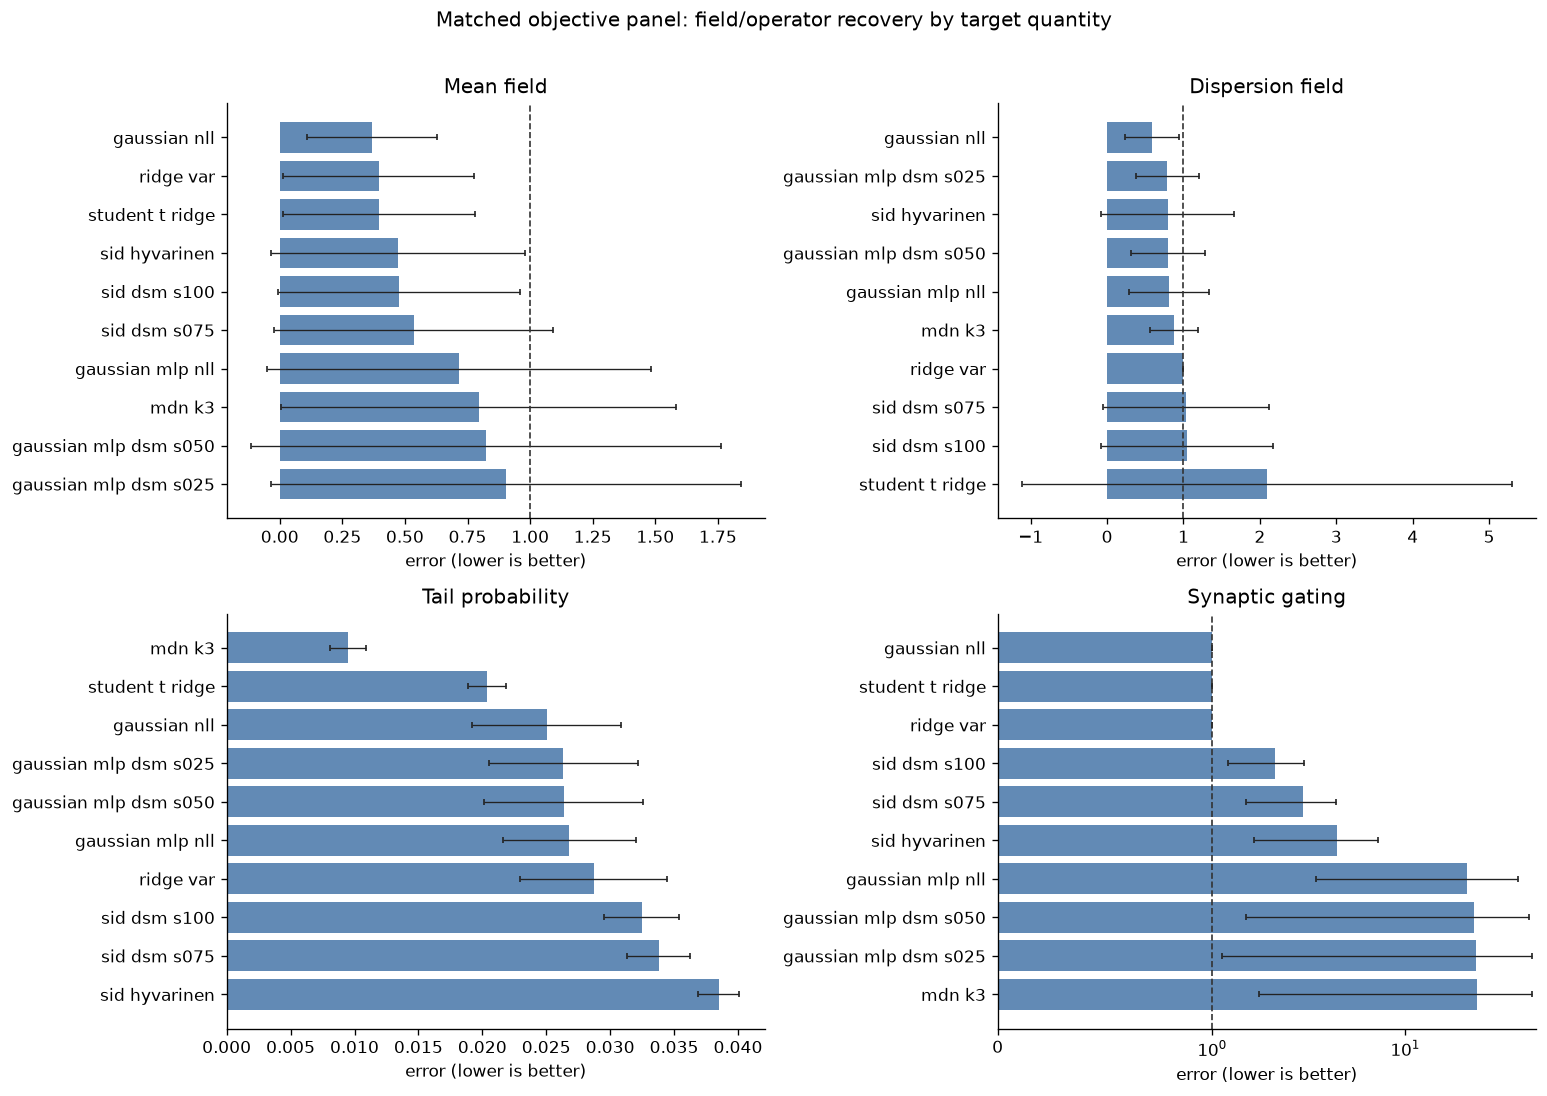
\includegraphics[width=0.93\linewidth]{../../analysis/synthetic_methods_adjudication/objective_parity.png}
  \caption{Matched objective comparison. Methods should be read by estimand: held-out law quality, mean-field recovery, and dispersion-field recovery are different tasks.}
  \label{fig:objective}
\end{figure}

For the physical additive-mean field in the new matched panel:

\begin{center}
\begin{tabular}{@{}lr@{}}
\toprule
Method & Mean-field \(\nise\) \\
\midrule
Penalized Gaussian NLL & \textbf{0.369} \\
Ridge Gaussian & 0.395 \\
Student-\(t\) ridge & 0.395 \\
Quadratic Hyv\"arinen SID & 0.473 \\
Quadratic DSM SID & 0.475--0.535 \\
Neural Gaussian NLL & 0.716 \\
MDN & 0.794 \\
Neural Gaussian DSM & 0.824--0.902 \\
\bottomrule
\end{tabular}
\end{center}

An earlier mechanism panel was even more favorable to classical dynamics: SINDy scored 0.194, sparse transition 0.201, Gaussian NLL 0.246, and Hyv\"arinen SID 0.268. The exact values differ across panels, but the ordering is consistent.

For the physical log-variance field:

\begin{center}
\begin{tabular}{@{}lr@{}}
\toprule
Method & Dispersion-field \(\nise\) \\
\midrule
Penalized Gaussian NLL & \textbf{0.586} \\
Neural Gaussian DSM, \(\sigma=.25\) & 0.789 \\
Quadratic Hyv\"arinen SID & 0.791 \\
Neural Gaussian DSM, \(\sigma=.50\) & 0.794 \\
Neural Gaussian NLL & 0.809 \\
MDN & 0.872 \\
Zero/constant-variance ridge & 1.000 \\
Quadratic DSM SID & 1.037--1.048 \\
Student-\(t\) ridge & 2.091 \\
\bottomrule
\end{tabular}
\end{center}

Neural DSM modestly improves over neural NLL within the same broad Gaussian architecture, so denoising may be a useful derivative regularizer. It does not beat the strictly parameterized Gaussian likelihood. This is evidence for a regularization effect, not a general score-objective advantage.

On the matched-tail law, representational flexibility matters:

\begin{center}
\begin{tabular}{@{}lrr@{}}
\toprule
Method & Held-out NLL & Tail-probability RMSE \\
\midrule
MDN, \(K=3\) & \textbf{-0.614} & \textbf{0.0095} \\
Student-\(t\) ridge & -0.530 & 0.0204 \\
Gaussian NLL & -0.288 & 0.0250 \\
Neural Gaussian DSM & -0.280 to -0.283 & 0.0263--0.0264 \\
Quadratic DSM SID & about -0.283 & 0.0325--0.0338 \\
Quadratic Hyv\"arinen SID & 9.18 & 0.0385 \\
\bottomrule
\end{tabular}
\end{center}

Yet the MDN's physical shape-tail derivative has \(\nise=2.02\), worse than the zero derivative. Predicting a tail probability and estimating its derivative with respect to a modulator are distinct problems.

\subsection{Synaptic gating: no current winner}

All nonzero learned readouts are worse than the zero field:

\begin{center}
\begin{tabular}{@{}lr@{}}
\toprule
Method & Total gating-field \(\nise\) \\
\midrule
Gaussian NLL / ridge / Student-\(t\), emit zero & \textbf{1.000} \\
Quadratic DSM SID & 2.10--2.95 \\
Quadratic Hyv\"arinen SID & 4.42 \\
Neural NLL / DSM / MDN & 20.97--23.40 \\
\bottomrule
\end{tabular}
\end{center}

The trajectories may contain gating, but the present fitted-law readout does not identify its mixed derivative reliably. More hyperparameter search over the same target is unlikely to change the conclusion. The next experiment must first show oracle identification from paired controlled laws or an explicitly gated transition model.

\subsection{History tangents and finite contrasts}

The infinitesimal point-history sweep completed 96 of 96 fits, passed fixed-batch overfit checks, and reproduced under exact replay. Nevertheless, six derivative-readiness gates failed. G1 location tangents reached NRMSE 0.589--0.719, while the best G2 covariance and G3 skew tangents were 1.068 and 1.167. The failure is therefore not explained by gross optimization failure.

\begin{figure}[t]
  \centering
  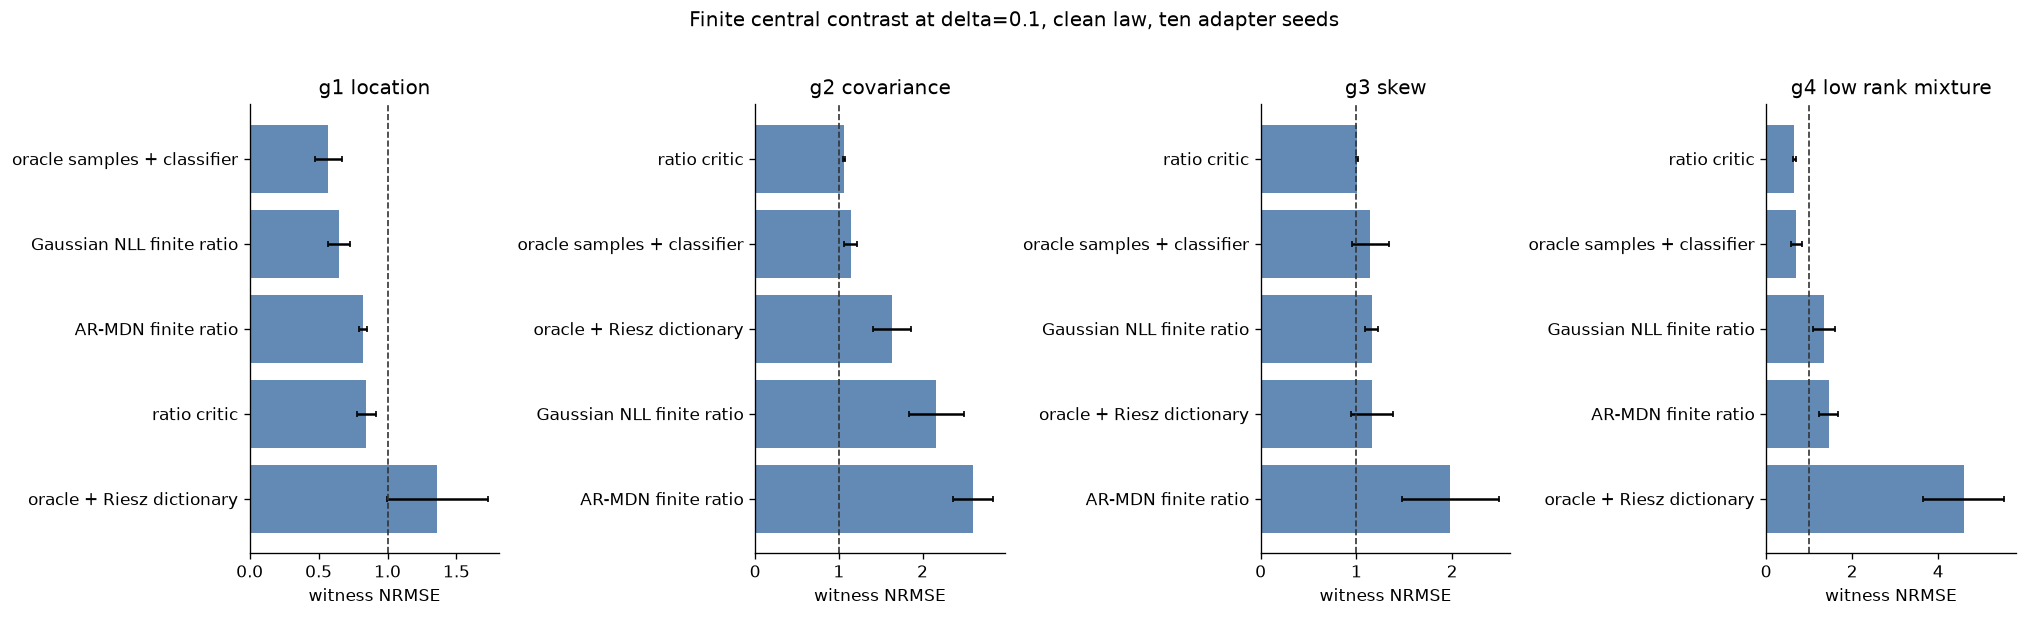
\includegraphics[width=0.98\linewidth]{../../analysis/synthetic_methods_adjudication/finite_contrast_ten_seed.png}
  \caption{Finite-contrast witness NRMSE across ten adapter/evaluation seeds at the main perturbation scale. The dashed reference at 1 is the zero-witness baseline.}
  \label{fig:finite}
\end{figure}

At clean \(\delta=0.1\), the ten-seed finite-contrast panel gives:

\begin{center}
\begin{tabularx}{0.96\linewidth}{@{}lXrX@{}}
\toprule
Generator & Best practically relevant route & Mean NRMSE & Verdict \\
\midrule
G1 location & Direct signed classifier / Gaussian finite ratio & about 0.61--0.65 & Useful; beats zero clearly \\
G2 covariance-only & Ratio critic & 1.057 & No recovery \\
G3 skew-only & Ratio critic & 1.008 & No recovery \\
G4 low-rank mixture & Ratio critic & \textbf{0.656} & Useful; beats zero clearly \\
\bottomrule
\end{tabularx}
\end{center}

The oracle infinitesimal tangent has negligible Taylor mismatch at this \(\delta\) for G2 and G3, but the oracle-sample classifier is still roughly 1.14 NRMSE. Consequently, the primary bottleneck is adapter geometry, response features, calibration, or signal-to-noise---not the learned diffusion generator. The current signed Riesz dictionary should not be scaled until an oracle redesign beats zero.

\subsection{SBTG localization}

The frozen SBTG panel shows joint-score cross-moment average-precision excess of roughly 0.15--0.39 for mean-like support. Similar values occur across additive, dispersion, and synaptic mechanisms, so the statistic is not mechanism-specific. Log-variance localization is only 0.06--0.10, and squared-score-covariance localization is roughly 0.00--0.05. Linear SBTG is often as good as or better than feature-bilinear variants.

The defensible conclusion is that SBTG can remain a reduced-form nonlinear screening/localization route. It has not established recovery of physical dispersion, gating, or a causal graph.

\subsection{Classical graph baselines and hidden confounding}

\begin{figure}[t]
  \centering
  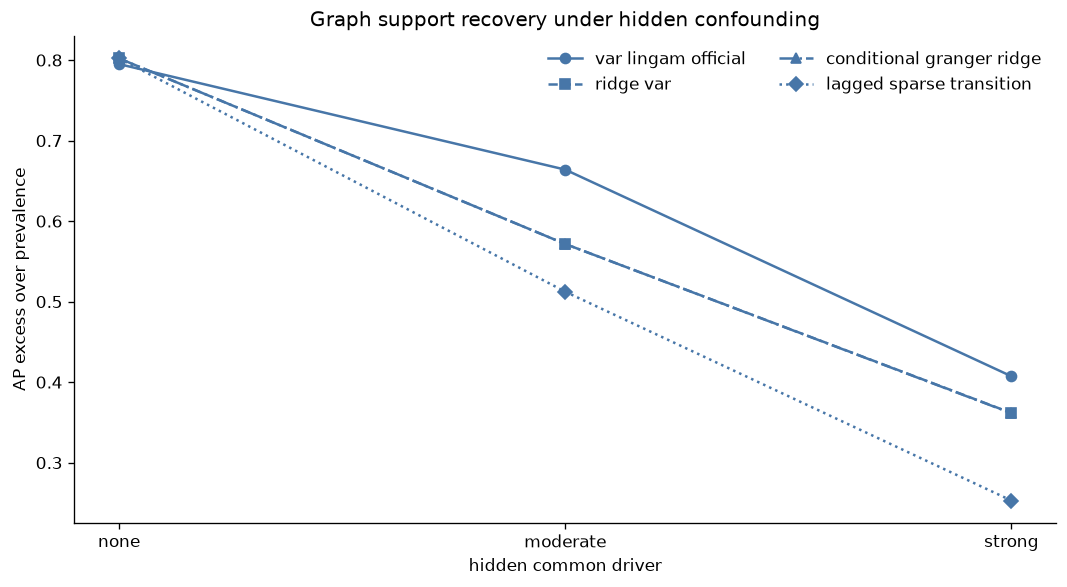
\includegraphics[width=0.74\linewidth]{../../analysis/synthetic_methods_adjudication/graph_hidden_confounding.png}
  \caption{Graph-support average-precision excess under causal sufficiency and strong hidden common drive. Every observational method degrades.}
  \label{fig:graph}
\end{figure}

Under causal sufficiency, classical transition methods reach about 0.80 AP excess. Under a strong hidden common driver, VAR-LiNGAM scores 0.407, ridge VAR 0.362, conditional Granger 0.361, PCMCI 0.338, sparse transition 0.253, and marginal lagged correlation 0.106. These are mandatory comparators. Even the best result is observational support recovery under a violated or stressed assumption, not identification of a latent causal mechanism.

\subsection{Changepoints}

With 199 matched-null calibration trajectories and 100 independent evaluation trajectories per condition:

\begin{itemize}
  \item the mean CUSUM detects and localizes 100/100 high-signal mean changes;
  \item the residual tail-shape probe detects and localizes 100/100 exactly mean/variance-matched tail changes;
  \item the residual variance probe calls 100/100 dispersion changes but localizes only 41/100;
  \item that variance probe also calls 95\% of mean changes and 99\% of matched-tail changes, so it is a broad residual-instability alarm rather than a dispersion-specific detector;
  \item independent-null false-positive rates are 2\% for mean, 4\% for conditional rule and variance, 3\% for tail, 9\% for MMD, and 11\% for energy distance.
\end{itemize}

Mean and tail provide strong matched demonstrations. Dispersion requires nuisance orthogonalization and confusion controls before it can carry a channel-specific label.

\section{Where our approaches have an advantage---and where they do not}

\subsection{Potential advantages}

The unified finite SID approach can be better than existing alternatives for reasons that are conceptual and testable:

\begin{enumerate}
  \item \textbf{Model-agnostic downstream interface.} The same contrast and readout can be applied to a tractable density, an energy model, a diffusion sampler, or an oracle simulator.
  \item \textbf{Exact finite estimand.} Equation~\eqref{eq:finite-witness} avoids pretending that an arbitrarily small derivative is scientifically meaningful or statistically stable.
  \item \textbf{Typed explanation of distributional change.} Unlike a single MMD or energy statistic, the witness can be integrated against declared mean, covariance, interaction, and tail features.
  \item \textbf{Bounded witness construction.} The absolute-coefficient mixture gives a bounded Radon--Nikodym witness, which is attractive for stable estimation and sequential concentration.
  \item \textbf{Multiple overidentifying routes.} Density ratios, classifiers, direct sample moments, and score reconstructions can target the same contrast. Agreement becomes a diagnostic rather than a rhetorical robustness check.
  \item \textbf{Resolution as a scientific parameter.} \(\delta\) specifies the perturbation being studied; \(\sigma\) specifies score corruption. Their effects can be separated and reported.
  \item \textbf{A path from local sensitivities to changes over time.} Once a channel is validated, the same typed statistic can be embedded in offline or online changepoint inference.
\end{enumerate}

\subsection{Costs and failure modes}

Those advantages come with real tradeoffs:

\begin{itemize}
  \item \textbf{Perturbation design:} the direction, magnitude, stencil, and support of \(T_{\delta,v}h\) are part of the estimand and may not be naturally identified from observational histories.
  \item \textbf{Overlap:} finite ratios and classifiers become unstable when \(P_{h_+}\) and \(P_{h_-}\) have little common support; tiny \(\delta\) has the opposite weak-signal problem.
  \item \textbf{Channel conditioning:} covariance, skew, and tail features can have high variance or poor geometry. An omnibus witness may be harder to learn than a direct targeted regression.
  \item \textbf{Derivative instability:} score or density convergence does not automatically imply convergence of derivatives with respect to history.
  \item \textbf{Corruption bias:} DSM learns a smoothed law. Fine changes can be attenuated by the denoising scale.
  \item \textbf{No causality for free:} predictive history dependence can arise from common drive, selection, or omitted state.
  \item \textbf{Computation:} multiple histories, routes, channels, and calibration blocks cost more than a single fitted transition model.
  \item \textbf{Baseline strength:} when the task really is conditional mean estimation under a sparse low-order law, ridge or SINDy is expected to win.
\end{itemize}

\subsection{When diffusion/score methods have a credible hope}

The present negative results do not imply that diffusion-based SID is hopeless. They imply that it needs a home-field experiment. A score/sample backend has a credible advantage when at least one of the following holds:

\begin{itemize}
  \item the conditional law is high-dimensional and multimodal, making normalized likelihood evaluation or integration impractical;
  \item the model is available only as a simulator or sampler;
  \item the scientific target depends on a local portion of response space that a mean/variance model erases;
  \item a shared generative model amortizes many contrasts or channels more efficiently than separately fitting targeted regressions;
  \item sample coupling or common noise can sharply reduce finite-difference variance.
\end{itemize}

To be impactful, the project must demonstrate one of these regimes. Beating a Gaussian likelihood on a near-Gaussian low-dimensional simulator is neither necessary nor likely. Conversely, merely functioning where likelihood is inconvenient is not enough; the method must yield a better estimand, better sample efficiency, or a capability the baseline cannot expose.

\section{Theory agenda}

The framework is conceptually coherent, but several results are needed to turn it into a mature method.

\subsection{Finite-witness stability bounds}

Derive error transfer from predictive laws or ratios to the witness and typed channels. Under overlap bounds and bounded \(\phi\), seek inequalities of the form
\[
  \left|\widehat\Delta_c(\phi)-\Delta_c(\phi)\right|
  \leq C_1\,d(\widehat P,P)+C_2\,\|\widehat W-W\|_{L^2(M)}
  +\text{sampling error},
\]
with explicit dependence on \(\delta\), dimension, and overlap. This would clarify when improving the predictive backend can actually improve the scientific readout.

\subsection{Bias--variance theory for \(\delta\) and \(\sigma\)}

Develop a phase diagram separating:

\begin{itemize}
  \item finite-stencil truncation bias as \(\delta\) grows;
  \item weak contrast and ratio variance as \(\delta\to0\);
  \item posterior smoothing/contraction as denoising noise \(\sigma\) grows;
  \item approximation and discretization error in reverse sampling.
\end{itemize}

The key theoretical question is whether the useful region scales with \(\sigma/\delta\), signal geometry, and intrinsic response dimension.

\subsection{Orthogonal and cross-fitted channel estimation}

Treat \(\Delta_c(\phi)\) as the primary low-dimensional functional and derive Neyman-orthogonal estimators using cross-fitted predictive laws and Riesz representers. This may allow slower nuisance convergence while retaining valid uncertainty for a small set of scientific channels. It is likely more promising for covariance and tail readouts than reconstructing the entire witness with a generic classifier.

\subsection{Reconstructing SID from SBTG}

Formalize the inverse problem in Equation~\eqref{eq:sbtg}. Given an estimate of \(K_v=\nabla_y\ell_v\), recover \(\ell_v\) by a weighted Poisson or Hodge problem with the conditional centering constraint
\[
  \int \ell_v(y;h)p_h(y)\,dy=0.
\]
Prove identifiability and stability under boundary/support assumptions. Compare this reconstruction against direct finite ratios at the oracle level. If the inverse problem is ill-conditioned in the tested regimes, SBTG should remain a localizer rather than the main SID route.

\subsection{Higher-order parity stencils}

Develop first- and second-order signed stencils whose finite witnesses are derived from the correct likelihood-ratio polynomial. A second derivative of a density includes both log-density Hessian and score-product terms; using a log Hessian alone generally targets the wrong signed measure. Establish exact coefficient/reference-mixture constructions and variance-optimal weighting.

\subsection{Route-agreement tests}

When density, classifier, direct-moment, and score routes target the same \(\Delta_c(\phi)\), formulate an overidentification test. Systematic disagreement can diagnose lack of overlap, score non-integrability, density calibration error, or sampler bias. This is potentially a distinctive contribution: the framework creates several estimators of one declared object rather than several incomparable model scores.

\subsection{Mechanism-confusion and nuisance invariance}

For a channel label to be meaningful, derive or enforce orthogonality to nuisance changes. A dispersion statistic should be insensitive to mean shifts; a standardized tail statistic should be insensitive to matched mean and variance changes. Develop residualization, influence-function, or adversarial nuisance-projection schemes and evaluate a full confusion matrix rather than only target power.

\subsection{Sequential inference}

Use bounded finite witnesses to construct blockwise e-values, martingales, or self-normalized scans under temporal dependence. The target result is false-alarm control across repeated monitoring while retaining a typed interpretation. Offline PELT and online BOCPD remain external inference engines; SID should contribute a validated cost or evidence sequence.

\section{The next decisive experiment program}

The next work should be staged. Later phases are conditional on earlier oracle gates; otherwise capacity and compute will obscure identification failures.

\subsection{Phase 0: oracle adapter tournament}

\textbf{Goal.} Determine whether each scientific channel is recoverable from perfect access to the relevant conditional laws before training any flexible predictive model.

\textbf{Data-generating families.}

\begin{itemize}
  \item G1: pure location change;
  \item G2: covariance-only rotation/scale change with fixed mean;
  \item G3: skew-only change with matched mean and covariance;
  \item G4: low-rank mixture interaction;
  \item mechanistic fields: additive mean, stochastic dispersion, matched tail, synaptic gating, and correlation-only changes.
\end{itemize}

\textbf{Oracle interfaces.} Exact log density and ratio where available; exact score; independent conditional samples; paired/common-random-number samples; exact moments; exact infinitesimal tangent.

\textbf{Adapters.}

\begin{itemize}
  \item exact finite ratio and direct log-ratio transformation;
  \item calibrated signed logistic classifier;
  \item KLIEP and uLSIF;
  \item polynomial/Hermite, kernel, and learned feature classifiers;
  \item channel-targeted Riesz estimators with cross-fitting;
  \item score-difference plus weighted Poisson/Hodge reconstruction;
  \item mixed SBTG operator plus the same reconstruction;
  \item direct paired-sample channel difference.
\end{itemize}

\textbf{Design.} At least 20 independent generator seeds, with separate data, adapter, and evaluation seeds. Sweep sample size, dimension, \(\delta\), overlap, and signal strength. The main perturbation scale is fixed before inspecting hard-channel results; other scales are sensitivity analyses.

\textbf{Primary metrics.} Witness NRMSE and channel nISE against the zero baseline of 1, with confidence intervals over generator seeds. Secondary metrics are calibration, centering, route disagreement, runtime, and effective sample size.

\textbf{Gate.} A channel advances only if at least one practical oracle adapter has an upper 95\% confidence bound below 1 and the intended channel is distinguishable from nuisance alternatives. G2/G3 currently fail this gate.

\subsection{Phase 1: backend \(\times\) adapter \(\times\) channel factorial}

\textbf{Goal.} Separate predictive-model error from adapter error and determine whether a shared flexible backend helps across multiple channels.

\begin{center}
\begin{tabularx}{\linewidth}{@{}p{0.19\linewidth}X@{}}
\toprule
Axis & Levels \\
\midrule
Backend & Oracle; ridge Gaussian; heteroskedastic Gaussian NLL; Student-\(t\); MDN; \SIDQ-Hyv\"arinen; \SIDQ-DSM; conditional score/diffusion; joint-score SBTG \\
Adapter & Direct density ratio; signed classifier; direct sample channels; Riesz; score/Hodge; mixed SBTG/Hodge \\
Channel & Mean; variance; covariance; low-rank interaction; skew; tail; local occupancy \\
Regime & Correct specification; heavy tails; mixtures; response coupling; high dimension; sample-only access \\
\bottomrule
\end{tabularx}
\end{center}

Every cell is evaluated on the same common estimand. Native NLL or DSM loss is reported only as a backend diagnostic. Exact seed intersections and identical train/validation/evaluation histories are required.

\textbf{Success criterion for diffusion.} A diffusion/score backend must either (i) beat the best feasible normalized backend on a common channel with uncertainty, or (ii) solve a sample-only/intractable-density task where the normalized comparator genuinely cannot expose the estimand, while beating direct empirical and generic two-sample baselines.

\subsection{Phase 2: scaling and stress map}

\textbf{Goal.} Find the regime, if any, where the unified approach has a real advantage.

Sweep:

\begin{itemize}
  \item sample size and effective dependent-block count;
  \item response dimension, history length, and intrinsic contrast rank;
  \item perturbation \(\delta\) and denoising scale \(\sigma\);
  \item observation noise, multimodality, tail weight, and support overlap;
  \item model misspecification and hidden common drive;
  \item number of requested channels/contrasts, to test amortization.
\end{itemize}

Report phase diagrams, not only aggregate ranks. The important question is where each method crosses NRMSE 1, how quickly it improves with data, and whether sharing a backend across many contrasts changes total cost.

\subsection{Phase 3: mechanism-confusion battery}

For every claimed channel, construct matched nuisances:

\begin{center}
\begin{tabular}{@{}lll@{}}
\toprule
Claimed channel & Positive condition & Mandatory negative/confusion conditions \\
\midrule
Mean & mean shift & variance, skew, tail, correlation changes \\
Dispersion & variance/scale change & mean, matched-tail, mixture-weight changes \\
Tail/shape & tail change matched in mean/variance & mean, variance, outlier contamination \\
Interaction & low-rank coupling change & marginal mean/variance changes \\
Graph/localization & edge-specific conditional change & common drive, indirect path, autocorrelation \\
\bottomrule
\end{tabular}
\end{center}

Report a confusion matrix of call rates and localization, not only target AUROC or AP.

\subsection{Phase 4: changepoints only for validated channels}

Carry forward only Phase 0--3 winners. Compare:

\begin{itemize}
  \item channel-specific CUSUM/GLR and PELT costs;
  \item MMD and energy-distance scans;
  \item BOCPD for online inference;
  \item bounded-witness e-value or martingale scans, if theory is ready.
\end{itemize}

Use independent matched-null calibration, independent evaluation, block resampling for dependence, and report false-positive rate, detection power, delay/detection-within-window, localization error, and mechanism confusion. Do not tune thresholds on the evaluation trajectories.

\subsection{Phase 5: long-horizon and pathwise extension}

Only after one-step typed contrasts are reliable, test block or rollout laws \(P(Y_{t+1:t+K}\mid H_t=h)\). Compare recursive and direct multi-horizon densities, conditional samplers, and paired pathwise contrasts. Vary horizon and coupling. The purpose is to learn whether finite SID effects compose or decay across time, not to introduce a separate latent mechanistic model.

\subsection{Preregistered decision rules}

\begin{enumerate}
  \item No learned-backend experiment for a channel whose practical oracle adapter fails the zero baseline.
  \item No downstream changepoint claim for a channel that fails static mechanism-confusion gates.
  \item No winner based only on native loss; all winners must beat baselines on a common population estimand.
  \item Independent generator, data, model-initialization, adapter, and evaluation seeds; exact seed intersections for pairwise comparisons.
  \item A simple zero/no-effect estimator is always included for normalized derivative metrics.
  \item One primary perturbation \(\delta\), corruption schedule, and metric per claim are fixed before evaluation.
  \item Report uncertainty over generator seeds, failure counts, calibration, compute, and route agreement.
  \item Preserve ridge, Gaussian/Student-\(t\) likelihood, MDN, SINDy, Granger/PCMCI/VAR-LiNGAM, MMD, energy, and appropriate changepoint baselines wherever their subproblem applies.
\end{enumerate}

\section{Research priorities and stop/go decisions}

\begin{center}
\begin{tabularx}{\linewidth}{@{}p{0.18\linewidth}p{0.15\linewidth}X X@{}}
\toprule
Direction & Priority & Why & Stop/go criterion \\
\midrule
Finite typed SID & Highest & Most coherent generalization; real G1/G4 wins; model-agnostic & Continue if redesigned oracle G2 or G3 adapter beats zero, or if robust G1/G4 scaling advantage appears \\
Targeted Riesz/orthogonal channels & High & Directly addresses hard covariance/tail functionals and uncertainty & Continue only after oracle cross-fitted estimator is stable and beats direct moment baselines \\
Diffusion as backend & Conditional/high & Needed for sample-only/high-dimensional laws, not low-dimensional Gaussian tasks & Continue if it wins a home-field task or enables a unique validated estimand \\
SBTG-to-SID reconstruction & Medium & Theoretically connects existing ideas and may yield local structure & Continue if oracle \(K_v\to\ell_v\) reconstruction is stable; otherwise retain as screen \\
Channel-specific changepoints & Medium after static gates & Strong mean/tail results; practical downstream use & Advance only validated channels with matched-null and confusion control \\
More \SIDQ sweeps & Low & Current objective parity is decisive on tested parametric tasks & Resume only for a new intractably normalized model or theory-motivated estimator \\
Generic gating mixed derivative & Stop/redesign & Every learned readout loses to zero & Require controlled paired identification or explicit gated parameterization first \\
\bottomrule
\end{tabularx}
\end{center}

\subsection{What would count as an impactful result?}

At least one of the following should be demonstrated:

\begin{itemize}
  \item a high-dimensional non-Gaussian conditional law where flexible-backend \FiniteSID beats feasible likelihood, direct moment regression, and generic two-sample methods on a common typed sensitivity;
  \item a sample-only setting where the framework reliably identifies a localized channel that density-based baselines cannot compute and direct empirical differences cannot estimate efficiently;
  \item a multi-contrast amortization result where one predictive generator plus SID adapters is substantially more accurate or efficient than separately trained targeted models;
  \item a calibrated changepoint system that both detects and correctly labels mean/dispersion/tail/interaction changes with controlled confusion under dependence;
  \item a theorem and experiment showing stable recovery of a centered SID witness from the SBTG mixed operator in a nontrivial class.
\end{itemize}

Without one of these, the framework may remain a useful organizational language but not yet a competitive method.

\section{Recommended paper-level narrative}

A future external paper should not claim that score matching generally outperforms likelihood or that a joint score reveals a causal mechanism. A defensible narrative is:

\begin{enumerate}
  \item Define predictive-law sensitivity through exact finite signed contrasts and typed channel functionals.
  \item Show that normalized densities, classifiers, scores, and samplers are interchangeable computational interfaces to the same estimand.
  \item Establish boundedness, stability, and uncertainty results for the finite witness and its channel readouts.
  \item Demonstrate oracle adapter validity, then learned-backend performance, in regimes where direct mean/variance models are insufficient.
  \item Use SBTG as a related gradient representation and changepoints as a downstream inference application.
  \item Be explicit that causal or mechanistic interpretations require extra assumptions or controlled perturbations.
\end{enumerate}

The strongest conceptual contribution is not a new loss. It is a typed, support-aware interface between predictive generative models and scientifically interpretable distributional sensitivities, together with tests that determine whether the interface is valid.

\section{Expanded out-of-family neuromodulation benchmark}
\label{sec:rethink-results}

The theory document motivates a substantially harder target than the earlier matched
complete-state benchmark: nonlinear high-dimensional dynamics, hidden modulators,
non-Gaussian and correlated innovations, calcium filtering and saturation, shared
artifact, partial observation, controlled operations, receptor kinetics, and
semi-Markov state paths. We therefore retained the earlier suite as a unit and
estimand-validation tier and executed a separate E1--E5 stress suite. No fitted method
received the hidden modulator or regime state.

The main run used 24 latent neurons, four hidden modulators, 12 training episodes, four
validation episodes, six test episodes, horizons 1, 4, and 16, and three independent
seeds. Seven fast methods ran in every cell. Gaussian and denoising neural networks,
an MDN, and feature-bilinear SBTG ran on a predeclared subset of 42 representative
stress cells. This produced 840 successful method--cell fits with no dropped failures.
A separate 32-neuron confirmation produced 672 successful fits for the full fast panel.

\subsection{Gaussian NLL is the empirical winner}

Table~\ref{tab:rethink-nll} reports average test negative log likelihood (lower is
better). Gaussian NLL ranks first in every scientific lane. This includes the
out-of-family nonlinear reservoir (E1), the paired measurement stress (E2), joint
noise/input/state/intervention shift (E3), stochastic release and receptor kinetics
(E4), and semi-Markov state dynamics (E5). The result persists at 32 neurons. Thus the
earlier Gaussian result was not only a consequence of giving a matched mechanistic
method the exact complete state, although the new generators remain bounded and the
available sample size still favors regularized low-complexity predictors.

\begin{table}[ht]
\centering
\caption{Mean test NLL in the 24-neuron expanded benchmark. Lower is better. Neural methods use their predeclared representative-cell panel and are not averaged over the same case mix as the fast methods.}
\label{tab:rethink-nll}
\begin{tabular}{@{}lrrrrr@{}}
\toprule
Method & E1 & E2 & E3 & E4 & E5 \\
\midrule
Gaussian NLL & 0.150 & -0.732 & -0.680 & -0.819 & -0.466 \\
Ridge VAR & 0.169 & -0.714 & -0.671 & -0.804 & -0.424 \\
Student-$t$ ridge & 0.255 & -0.645 & -0.600 & -0.728 & -0.331 \\
Gaussian MLP NLL & 0.203 & -0.229 & -0.628 & -0.663 & -0.386 \\
MDN & 0.206 & -0.217 & -0.608 & -0.634 & -0.393 \\
\bottomrule
\end{tabular}
\end{table}

Across all 96 fast-panel cells at 24 neurons, Gaussian NLL improves on ridge VAR by
0.0187 NLL units on average and wins 76.0\% of paired cells. At 32 neurons its advantage
increases to approximately 0.055 NLL units and it wins approximately 95\% of comparable
cells. With only three independent simulator seeds these are repeated-condition
summaries, not a precise population confidence interval. Seed-level Gaussian-NLL skill
over ridge is 0.001, 0.039, and 0.014 at 24 neurons, and 0.064, 0.031, and 0.070 at 32
neurons.

The nonlinear density models do not exploit a decisive advantage at this data scale.
Gaussian MLP, DSM-trained Gaussian MLP, and MDN remain valid but generally trail the
linear Gaussian likelihood. SBTG is a score-only model and is therefore excluded from
the NLL table rather than assigned a fictitious likelihood. Its held-out DSM risk is
finite across all 42 cells, but that native loss cannot establish predictive-law or
typed-channel superiority over normalized-density baselines.

\subsection{Unconstrained quadratic SID fails expected-risk and stability gates}

The quadratic SID median fit can appear reasonable, but its expected predictive risk is
not. At 24 neurons, the Hyv\"arinen and DSM variants pass their own numerical-validity
diagnostic in 90.6\% and 92.7\% of cells, respectively. At 32 neurons these rates fall to
82.3\% and 90.6\%. Rare crossings of the natural-variance boundary create extremely
large means or variances, so mean NLL and mean normalized RMSE become catastrophic even
when median NLL looks ordinary. This is not a cosmetic outlier issue: a probabilistic
model used for forecasting or likelihood comparison must control expected loss.

A post-benchmark diagnostic fit 432 additional SID models across 18 representative
E1--E5 cells, crossing six ridge values and four corruption scales. Ridge 1 with DSM
corruption $\sigma=1$ was the best validity-first setting: 100\% validity, median NLL
$-0.526$, mean NLL $-0.351$, and mean normalized RMSE 0.769. The matched ridge-VAR mean
NLL was $-0.435$. Ordinary tuning therefore can stabilize the implementation, but it
does not make SID win. Moreover, some settings marked formally valid still had extreme
RMSE, showing that the present diagnostic is weaker than the desired deployment gate.

The theoretical implication is constructive: retain the score-identified estimands,
but replace the unconstrained quadratic natural-variance map with a parameterization
that enforces positive, bounded-away-from-zero scale and controls tail behavior by
construction. A constrained log-scale model, calibrated fallback, or normalized
density backend may serve SID readouts without inheriting this failure mode.

\subsection{Paired intervention response favors direct regularized dynamics}

E3 and E4 include common-random-number control and operated trajectories. We evaluate
the difference between predicted operated and control outcomes against the true paired
difference. Averaged across active operations, ridge, heteroskedastic ridge, and
Student-$t$ ridge tie at response NRMSE 0.189; Gaussian NLL scores 0.194;
DSM-SID 0.202; Hyv\"arinen SID 0.210; and the zero-response baseline 0.293. The methods
capture part of the response through the evolving observed history, but all attenuate
its magnitude. No current SID method has an intervention-transfer advantage.

These response estimates are reduced-form. E4 uses stochastic release, saturating
occupancy, adaptation, and receptor attenuation, but good fluorescence forecasting does
not identify a unique ligand--receptor mechanism. Likewise, E5 establishes predictive
performance under modulator-dependent semi-Markov switching; a dedicated HMM/HSMM
state-recovery tournament remains necessary before claiming state or dwell-law recovery.

\subsection{Updated decision}

The expanded benchmark changes the priority ordering.

\begin{enumerate}
  \item Use Gaussian NLL and ridge as mandatory baselines and current practical defaults.
  \item Stop treating unconstrained quadratic SID as a deployable predictive law.
  \item Preserve finite typed SID contrasts as the main theoretical contribution, but
        compute them from a stable normalized density, direct ratio/classifier, or a
        positivity-constrained score backend.
  \item Continue diffusion only in a declared home field---multimodal, implicit, or
        sample-only conditional laws---and require it to beat MDN/flow/direct-ratio
        baselines there.
  \item Add explicit HMM/HSMM and direct response-kernel baselines before elevating the
        E5 path-law or E4 mechanistic claims.
\end{enumerate}


\section{Final answer to the strategic questions}

\textbf{Which of our methods works best?} On the expanded out-of-family synthetic evidence, Gaussian NLL is the best conditional-law estimator and ridge is the best or equal-best response-contrast estimator. Among the project's original score/SID ideas, finite supported contrasts remain the most credible direction: signed classifier or finite ratio routes are useful for location, and ratio critics are useful for low-rank mixture interactions. Mean and matched-tail changepoint probes are strong downstream results. Unconstrained quadratic \SIDQ and SBTG do not currently beat the appropriate baselines broadly.

\textbf{Do the non-winners have hope?} Yes, but only with sharper conditions. A post-benchmark sweep shows that strong regularization and large corruption can stabilize quadratic SID, but the stabilized fit still loses to ridge on mean NLL. The immediate problem is therefore not merely tuning: positivity and tail control should hold by construction. Diffusion-SID still has a plausible home field in genuinely multimodal, intractably normalized, or sample-only laws, but that advantage has not yet been demonstrated. SBTG has hope as a local derivative representation if a stable reconstruction to the centered history witness can be proved and demonstrated. Covariance/skew channels have hope only after an oracle adapter redesign; more predictive-model training cannot fix an adapter that fails with oracle samples. Generic gating readouts should be stopped until the identification design changes.

\textbf{Where are we going?} Toward finite, typed, support-aware SID rather than toward one universal score objective. The next milestone is an oracle adapter tournament with strict gates, followed by a backend-by-adapter factorial in a deliberately chosen home-field regime for flexible generative models. Static validity precedes changepoints. Classical baselines remain first-class competitors.

\appendix

\section{Reproducibility and evidence map}

This synthesis concerns theory and synthetic data only. Real neural-data performance is intentionally outside scope. The principal local evidence sources are:

\begin{itemize}
  \item \path{SYNTHETIC_METHODS_REPORT_2026-07-12.md}: prior adjudication and exact result summaries;
  \item \path{analysis/synthetic_methods_adjudication_2026-07-12.ipynb}: executed analysis notebook;
  \item \path{analysis/synthetic_methods_adjudication/method_taxonomy.csv}: method inventory;
  \item \path{neuromod_benchmark/configs/objective_adjudication_20260712.yaml}: matched objective configuration;
  \item \path{neuromod_benchmark/outputs/objective_adjudication_20260712/}: 250-case matched objective outputs;
  \item \path{history_tangent_benchmark/results/revised_note_v1_finite_contrast_20260712_seed5004} through \path{seed5013}: ten-seed finite contrast outputs;
  \item \path{neuromod_benchmark/outputs/rethink_suite_20260712_v2/}: 24-neuron E1--E5 run with neural and score-model panel (840 fits);
  \item \path{neuromod_benchmark/outputs/rethink_suite_20260712_n32_fast/}: 32-neuron scale confirmation (672 fits);
  \item \path{neuromod_benchmark/outputs/rethink_suite_20260712_sid_stability/}: 432-fit SID regularization/corruption diagnostic;
  \item \path{neuromod_benchmark/docs/THEORY.md} and \path{neuromod_benchmark/docs/METRIC_CONTRACT.md}: estimands, claim ladder, and metric contract;
  \item \path{tmp/pdfs/SBTG_Revised_Technical_Note_July_2026.txt}: revised predictive-generator and finite-witness theory note.
\end{itemize}

Software checks at the time of the adjudication passed 247 neuromod benchmark tests and 57 history-tangent tests. Passing tests establishes implementation consistency, not scientific identification; the oracle and baseline gates in this report are stricter.

\section{Compact claim ladder}

\begin{center}
\begin{tabularx}{\linewidth}{@{}p{0.18\linewidth}X X@{}}
\toprule
Claim type & What is supported & What is not implied \\
\midrule
Predictive law & Held-out conditional distribution fit & Correct derivatives or physical mechanism \\
Finite contrast & Difference between declared supported histories & Infinitesimal effect outside the stencil; causal intervention \\
Typed channel & Change in a declared response feature & Other channels or a unique mechanism \\
Localization/graph & Reduced-form predictive dependence support & Causal edge under hidden confounding \\
Changepoint & Calibrated detection/localization of a statistic change & Mechanism label unless confusion gates pass \\
\bottomrule
\end{tabularx}
\end{center}

\begin{thebibliography}{99}

\bibitem{hyvarinen2005}
A. Hyv\"arinen.
Estimation of non-normalized statistical models by score matching.
\emph{Journal of Machine Learning Research}, 6:695--709, 2005.
\url{https://jmlr.org/papers/v6/hyvarinen05a.html}

\bibitem{vincent2011}
P. Vincent.
A connection between score matching and denoising autoencoders.
\emph{Neural Computation}, 23(7):1661--1674, 2011.
\url{https://doi.org/10.1162/NECO_a_00142}

\bibitem{song2021}
Y. Song, J. Sohl-Dickstein, D. P. Kingma, A. Kumar, S. Ermon, and B. Poole.
Score-based generative modeling through stochastic differential equations.
\emph{International Conference on Learning Representations}, 2021.
\url{https://arxiv.org/abs/2011.13456}

\bibitem{kanamori2009}
T. Kanamori, S. Hido, and M. Sugiyama.
A least-squares approach to direct importance estimation.
\emph{Journal of Machine Learning Research}, 10:1391--1445, 2009.
\url{https://jmlr.org/papers/v10/kanamori09a.html}

\bibitem{gretton2012}
A. Gretton, K. M. Borgwardt, M. J. Rasch, B. Sch\"olkopf, and A. Smola.
A kernel two-sample test.
\emph{Journal of Machine Learning Research}, 13:723--773, 2012.
\url{https://jmlr.org/papers/v13/gretton12a.html}

\bibitem{brunton2016}
S. L. Brunton, J. L. Proctor, and J. N. Kutz.
Discovering governing equations from data by sparse identification of nonlinear dynamical systems.
\emph{Proceedings of the National Academy of Sciences}, 113(15):3932--3937, 2016.
\url{https://doi.org/10.1073/pnas.1517384113}

\bibitem{runge2019}
J. Runge, P. Nowack, M. Kretschmer, S. Flaxman, and D. Sejdinovic.
Detecting and quantifying causal associations in large nonlinear time series datasets.
\emph{Science Advances}, 5(11):eaau4996, 2019.
\url{https://doi.org/10.1126/sciadv.aau4996}

\bibitem{hyvarinen2010}
A. Hyv\"arinen, K. Zhang, S. Shimizu, and P. O. Hoyer.
Estimation of a structural vector autoregression model using non-Gaussianity.
\emph{Journal of Machine Learning Research}, 11:1709--1731, 2010.
\url{https://jmlr.org/papers/v11/hyvarinen10a.html}

\bibitem{pamfil2020}
R. Pamfil, N. Sriwattanaworachai, S. Desai, P. Pilgerstorfer, K. Georgatzis, P. Beaumont, and B. Aragam.
DYNOTEARS: Structure learning from time-series data.
\emph{Proceedings of AISTATS}, PMLR 108:1595--1605, 2020.
\url{https://proceedings.mlr.press/v108/pamfil20a.html}

\bibitem{chernozhukov2022}
V. Chernozhukov, W. K. Newey, and R. Singh.
Automatic debiased machine learning of causal and structural effects.
\emph{Econometrica}, 90(3):967--1027, 2022.
\url{https://doi.org/10.3982/ECTA18515}

\bibitem{killick2012}
R. Killick, P. Fearnhead, and I. A. Eckley.
Optimal detection of changepoints with a linear computational cost.
\emph{Journal of the American Statistical Association}, 107(500):1590--1598, 2012.
\url{https://doi.org/10.1080/01621459.2012.737745}

\bibitem{adams2007}
R. P. Adams and D. J. C. MacKay.
Bayesian online changepoint detection.
Technical report, 2007.
\url{https://arxiv.org/abs/0710.3742}

\end{thebibliography}

\end{document}
